\documentclass[mpi]{exam}
\usepackage{code}
\usepackage{base}
\usepackage{makecell}
\usepackage{multicol}
\usepackage{enumitem}
% \setlist{leftmargin=3mm}

\title{QCM MPI corrigé}

\begin{document}

Les réponses correctes sont exactement celles en gras. Des commentaires sont en italique.
\begin{multicols}{1}  

\section*{Structures de données}

\begin{enumerate}
    \item À quoi s'évalue l'expression \ocaml{0.1 +. 0.2 = 0.3} en OCaml ?
    \begin{enumerate}
        \item Une erreur car il faut utiliser \ocaml{==}.
        \item Une erreur car il faut utiliser \ocaml{=.} sur des flottants.
        \item \blacktriangleright \ocaml{false} car \ocaml{0.1} est stocké de façon approchée. \textit{Les flottants sont stockés en base 2 et 0.1 n'a pas d'écriture exacte en base 2. Il y a donc des erreurs d'arrondis.}
        \item \ocaml{true} car \ocaml{0.1 +. 0.2} est égal à \ocaml{0.3}.
    \end{enumerate}
    \item La suite de bits $11101100$ peut a priori représenter ... 
    \begin{enumerate}
        \item Un entier naturel plus grand que $1000$. \textit{Au maximum sur $8$ bits on représente les entiers de l'intervalle $\llbracket 0, 2^8 -1 \rrbracket = \llbracket 0, 255 \rrbracket$. \`A moins d'introduire une façon très atypique de représenter les entiers...}
        
        \item \blacktriangleright {Un entier strictement négatif.} \textit{Représente $-2^7 +2^6+2^5+2^3+2^2 = -20$ en complément à 2.}
        \item \blacktriangleright {Un rationnel.} \textit{Cette suite peut représenter un flottant, même si on ne peut pas savoir lequel exactement car on ne sait pas combien de bits sont utilisés pour l'exposant et combien pour la mantisse.}
        \item \blacktriangleright {Un caractère.} \textit{Oui, mais attention on est au delà de $127$ donc ce n'est plus un caractère ASCII.}
    \end{enumerate} 
    \item Un pile est ... 
        \begin{enumerate}
            \item \blacktriangleright {Une structure FILO (First In, Last Out)}. \textit{On peut aussi dire LIFO (Last In, First Out).}
            \item Une structure FIFO (First In, First Out). \textit{C'est une file.}
            \item \blacktriangleright {Une structure disponible nativement en OCaml.} \textit{On peut utiliser une liste pour implémenter une pile.}
            \item \blacktriangleright {Utile pour implémenter un parcours en profondeur.} \textit{C'est une alternative au DFS par fonction récursive : dans un while, on dépile, on traite le sommet, et on empile les voisins non visités.}
            \item Utile pour implémenter un parcours en largeur.
        \end{enumerate}
    \item Une file peut ...
        \begin{enumerate}
            \item \blacktriangleright {\^Etre implémentée par deux piles avec des opérations élémentaires en temps constant (en complexité amortie).} \textit{Le sommet de la pile 1 est la tête de file et celui de la pile 2 est sa queue. La création créé deux piles vides en temps constant, l'ajout est en temps constant, le retrait demande parfois de transvaser pile 2 dans pile 1.}
            \item \^Etre implémentée par une seule pile. \textit{On a besoin de savoir où est la tête et où est la queue.}
            \item Utile pour implémenter un parcours en profondeur.
            \item \blacktriangleright {Utile pour implémenter un parcours en largeur.}
            \end{enumerate}
    \item Une fonction de hachage peut être utilisée ...
        \begin{enumerate}
            \item \blacktriangleright {En sécurité informatique.}
            \item \blacktriangleright {Pour la reconnaissance de motif dans un texte.} \textit{Dans l'algorithme de Rabin-Karp.}
            \item \blacktriangleright {Pour la mémoïsation.} \textit{Pour implémenter un dictionnaire via table de hachage.}
            \item Pour accélérer l'algorithme des $k$ plus proches voisins. \textit{Non, mais en revanche la recherche des $k$ plus proches voisins d'un points peut être accélérée par l'utilisation d'arbres $d$-dimensionnels.}
        \end{enumerate}
    \item Quelles structures sont persistantes ? \textit{On rappelle que persistant/fonctionnel veut dire non-modifiable, contrairement à mutable/impératif}
        \begin{enumerate}
            \item \blacktriangleright {Liste OCaml.}
            \item Tableau.
            \item \blacktriangleright {Arbre binaire OCaml.}
            \item Tas binaire.\textit{L'implémentation classique utilise un tableau}
            \item Chaîne de caractères en C.\textit{Tableau de char}
            \item \blacktriangleright {Chaîne de caractères en OCaml}.\textit{Autre implémentation qu'en C}
        \end{enumerate} 
    \item Si on considère un arbre binaire strict et non vide à $n$ noeuds internes, $f$ feuilles et de hauteur $h$, quelles relations sont vérifiées parmi les suivantes ?
        \begin{enumerate}
            \item $f \leq n$. \textit{Considérer un arbre à un noeud : $f = 1$ et $n = 0$.}
            \item $f+n < 2^{h+1}-1.$ \textit{Est faux sur une racine : $f +n = 1+0 = 1 = 2^{0+1}-1$. L'inégalité large est vraie.}
            \item \blacktriangleright ${n \geq h}$.
            \item \blacktriangleright ${f = n+1}$. \textit{Se démontre par récurrence sur la taille par exemple.}
            \item \blacktriangleright ${f+n+h \neq 0}$. \textit{Puisque l'arbre est non vide.}
        \end{enumerate}
    \item En ignorant la valeur des étiquettes des noeuds, combien y a-t-il d'arbres binaires de hauteur exactement $2$~? 
        \begin{enumerate}
            \item $3$.
            \item $14$.
            \item \blacktriangleright ${21}$. \textit{Il y a un arbre de hauteur $-1$, un de hauteur $0$ et trois de hauteur $1$. Dans un arbre de hauteur $2$, l'un des fils doit être de hauteur 1 et l'autre est quelconque parmi les $5$ possibles. L'ensemble $G$ des arbres binaires de hauteur $2$ dont le fils gauche est de hauteur $1$ contient donc $15$ éléments (donc plus que $14$) et si on fixe le fils droit comme étant de hauteur $2$, on a au maximum $15$ arbres supplémentaires, et en fait moins, car certains sont déjà présents dans $G$. En tous cas, on en a moins que $15 + 15 = 30$. C'est donc la bonne réponse par élimination et on peut le vérifier en dessinant tous les arbres.}
            \item $35$.
        \end{enumerate}
    \item Le parcours en largeur d'un arbre est ...
        \begin{enumerate}
            \item \blacktriangleright {Linéaire en le nombre de noeuds.}
            \item \blacktriangleright {Linéaire en le nombre d'arêtes.} \textit{Dans un arbre, $a = n-1$ donc une quantité est linéaire en le nombre $n$ de noeuds si et seulement si elles est linéaire en le nombre $a$ d'arêtes.}
            \item Linéaire en la hauteur. \textit{Pas dans un arbre complet par exemple.}
            \item Jamais utilisé en pratique.
            \item L'ordre inverse du parcours en profondeur.
        \end{enumerate}
    \item On note $r(a)$ la racine d'un arbre $a$. Soit $a$ un arbre binaire non vide et de sous-arbres $g$ et $d$. On suppose que les éléments de $a$ sont tous différents. Quelle(s) proposition(s) suivante(s) sont équivalentes à << $a$ est un arbre binaire de recherche (ABR) >> ? \textit{Il faut que tous les éléments de $g$ soient inférieurs à $r(a)$, tous les éléments de $d$ supérieurs à $r(a)$, $g$ ABR et $d$ ABR. On peut trouver des contre-exemples pour les autres propositions.}
            \begin{enumerate}
                \item $r(g) < r(a)$, $r(d) < r(a)$, et $g$, $d$ sont des ABR.
                \item $r(g) < r(a) < r(d)$, et $g$, $d$ sont des ABR. 
                \item Tous les éléments de $g$ sont inférieurs à $r(a)$ et tous les éléments de $d$ sont supérieurs à $r(a)$.
                \item \blacktriangleright {Le parcours infixe de $a$ est croissant.}
                \item Le parcours préfixe de $a$ est croissant.
            \end{enumerate}
    \item Dans un arbre binaire de recherche de taille $n$ et de hauteur $h$, on peut ... 
        \begin{enumerate}
            \item \blacktriangleright {Trouver un élément en $O(n)$.} \textit{Puisque $h \leq n$.}
            \item \blacktriangleright {Trouver un élément en $O(h)$.}
            \item Trouver un élément en $O(\log n)$. \textit{La recherche dans un ABR est linéaire en sa hauteur. Si l'arbre n'est pas équilibré, cette hauteur peut être de l'ordre de $n$ donc cette opération n'est pas en $O(\log n)$.}
            \item Insérer un élément en $O(\log n)$. \textit{Idem (C) car l'insertion est aussi en $O(h)$.}
            \item Supprimer un élément en $O(\log n)$. \textit{Idem (C) car la suppression est aussi en $O(h)$.}
            \item \blacktriangleright {Vérifier qu'il est bien ABR en $O(n)$.} \textit{Il suffit d'en faire le parcours infixe et de vérifier qu'il est trié. Attention, si on regarde naïvement si la racine est plus grande que le max à gauche, plus petite que le min à droite et que les deux fils sont ABR, l'analyse de complexité est plus délicate.}
        \end{enumerate}
    \item Les arbres rouge-noir ... \textit{Rappel : un arbre rouge-noir est un ABR strict dont la racine est noire (les feuilles vide aussi), les fils d'un noeud rouge sont noirs et tel que tous les chemins de la racine à une feuilles ont autant de noeuds noirs. L'insertion et la suppression utilisent des rotations.}
        \begin{enumerate}
            \item \blacktriangleright {Sont des ABR.}
            \item \blacktriangleright {Peuvent être utilisés pour implémenter un dictionnaire.} \textit{C'est l'un des intérêts d'un ABR.}
            \item N'assurent aucune garantie de complexité. \textit{Au contraire puisqu'un arbre rouge-noir est équilibré.}
            \item N'ont pas d'utilité pratique.
            \item \blacktriangleright {Nécessitent un bit d'information supplémentaire par noeud par rapport à un arbre binaire.} \textit{\`A savoir la couleur du noeud.}
            \item Ne peuvent pas stocker de valeurs.
        \end{enumerate}
    \item La structure de tas peut être utilisée dans les algorithmes suivants ... 
        \begin{enumerate}
            \item \blacktriangleright {Algorithme de Kruskal.} \textit{Un peu abusif : si on utilise un tri par tas pour trier les arêtes.}
            \item Algorithme de parcours en profondeur. 
            \item Algorithme de Kosaraju.
            \item \blacktriangleright {Algorithme du tri par tas.} \textit{\'Evidemment.}
            \item \blacktriangleright {Algorithme de Dijkstra.} \textit{Via la file de priorité qui gère quel sommet étudier.}
        \end{enumerate}
    \item Il existe une implémentation de la structure unir et trouver ayant une complexité ... 
        \begin{enumerate}
            \item \blacktriangleright {Constante pour l'opération unir.} \textit{On représente les classes par les composantes connexes d'un graphe représenté par matrice d'adjacence. Unir revient à ajouter une arête ce qui se fait en temps constant. Trouver consiste (par exemple) à parcourir la composante pour en trouver le plus petit élément.}
            \item \blacktriangleright {Constante pour l'opération trouver.} \textit{Via un tableau stockant le numéro de partition de $i$ en case $i$.}
            \item Constante pour l'opération trouver et l'opération unir.
            \item Constante en complexité amortie pour l'opération trouver et l'opération unir. \textit{Même avec union par rang et compression de chemin, la complexité amortie n'est pas constante mais en $O(\alpha(n))$. On peut juste dire "en pratique on peut la considérer constante".}
            \item \blacktriangleright {En $O(\log n)$ dans le pire cas pour les opérations trouver et unir où $n$ est le nombre d'éléments manipulés.} \textit{Via une forêt avec union par hauteur.}
        \end{enumerate}
    \item Un graphe est régulier si tous ses sommets ont le même degré. Existe-t-il un graphe régulier ayant ...
        \begin{enumerate}
            \item \blacktriangleright {$9$ sommets.} \textit{Avec un graphe à $9$ sommets sans arêtes par exemple.}
            \item \blacktriangleright {Degré $5$ avec $3$ composantes connexes.} \textit{Juxtaposer $3$ fois le graphe complet à $6$ sommets.}
            \item Degré $5$ avec $9$ sommets. \textit{Impliquerait que $2|A| = \sum \deg(s) = 9 \times 5 = 45$ donc que $45$ est pair.}
            \item Degré $6$ avec $6$ sommets. \textit{Chaque sommet ne peut être relié qu'à $5$ sommets dans un graphe à $6$ sommets.}
            \item \blacktriangleright {Un degré $p$ et un nombre $q$ de sommets avec des $p$ et $q$ premiers.} \textit{Le graphe complet à $3$ sommets convient ($p = 2$). On ne demande pas ici si on a un graphe régulier pour tous $p$ et $q$ premiers.}
        \end{enumerate}
    \item L'ensemble des graphes orientés à $n$ sommets ...
    \textit{Il y a $n(n-1)$ arcs possibles dans un graphe orienté à $n$ sommets puisqu'un arc est une paire de sommets distincts. Chaque partie de cet ensemble à $n(n-1)$ éléments donne naissance à exactement un graphe orienté : il y en a donc $2^{n(n-1)}$.} 
        \begin{enumerate}
            \item Est en bijection avec l'ensemble des graphes non orientés à $n$ sommets. \textit{Dans un graphe non orienté il y a $k = n(n-1)/2$ arêtes possibles donc $2^k$ graphes possibles.}
            \item Est en bijection avec l'ensemble des graphes non orientés à $\lceil n/2 \rceil$ sommets. \textit{Avec les raisonnements précédents, il y a $2^{\lceil n/2 \rceil (\lceil n/2 \rceil -1)/2}$ tels graphes.}
            \item Est en bijection avec le groupe symétrique $S_n$. \textit{Cet ensemble est de cardinal $n!$.}
            \item \blacktriangleright {Est en bijection avec l'ensemble des mots de $\{a,b \}^{n^2-n}$.} \textit{Correct puisque pour construire un mot sur $\{a,b \}$ de longueur $n^2 - n$, on a deux possibilité pour chacune des $n^2-n$ positions.}
            \item Est en bijection avec l'ensemble des langages qui contiennent $n$ mots sur $\{a,b\}$. \textit{Cet ensemble n'est pas fini puisque les langages $L_i = \{a^i, a^{i+1}, ..., a^{i+n-1} \}$ en sont et sont tous différents.}
        \end{enumerate}
    \item Un graphe non orienté à $m$ arêtes et $n$ sommets est un arbre si et seulement si ... 
        \begin{enumerate}
            \item Il est acyclique. \textit{Contre-exemple : un graphe acyclique non connexe.}
            \item \blacktriangleright {Il est acyclique avec $m = n-1$.}
            \item Il possède une racine.
            \item \blacktriangleright {Toute paire de sommets est reliée par un unique chemin.}
            \item \blacktriangleright {Il est connexe avec $m < n$.} \textit{Un arbre vérifie cette propriété. Réciproquement, tout graphe connexe vérifie $m \geq n-1$. Comme $m <n$, on a donc un graphe connexe avec $m = n-1$ ce qui caractérise bien un arbre.}
        \end{enumerate}
    \item La complexité d'un parcours en profondeur du graphe $G = (S,A)$ est ... 
        \begin{enumerate}
            \item En $O(|S|^2)$ quelle que soit la représentation du graphe. \textit{Sauf peut-être si on s'autorise un précalcul en $O(|S|^2)$ pour transformer la représentation choisie en une autre plus adéquate.}
            \item En $O(|A|)$ si $G$ représenté par listes d'adjacence. \textit{$O(|S| + |A|)$ : il faut initialiser le tableau des vus.}
            \item \blacktriangleright {En $O(|S|^2)$ si $G$ est représenté par matrice d'adjacence.} 
            \item En $O(|S| + |A|)$ si $G$ est représenté par matrice d'adjacence. \textit{Car le calcul des voisins d'un sommet $s$ demande de l'ordre de $|S|$ opérations à la place de $\deg s$ avec listes d'adjacence.}
            \item En $O(|S|+|A|)$ si $G$ est représenté par liste d'arêtes. \textit{Techniquement oui car on peut convertir une représentation par liste d'arêtes en une représentation par listes d'adjacence en temps $O(|S| + |A|)$.}
        \end{enumerate}
\end{enumerate}


\section*{Algorithmique}

\begin{enumerate}[resume]
    \item Un invariant de boucle ... 
        \begin{enumerate}
            \item \blacktriangleright {Aide à prouver la correction d'un algorithme.}
            \item Est vérifié si et seulement si la propriété reste vraie après une itération si on la suppose vraie avant. \textit{Il faut aussi que la propriété soit vraie avant la toute première itération de la boucle (initialisation).}
            \item \blacktriangleright {Est vérifié en sortie de boucle.} \textit{On entend ici "invariant" au sens de "propriété dont on a montré qu'elle est bien un invariant de boucle" et pas "propriété dont il faut encore montrer qu'elle est invariante.}
            \item Correspond à une formulation de la correction de l'algorithme sur des sous-problèmes.
            \item Aucune des propositions ci-dessus.
        \end{enumerate}
    \item Un algorithme qui termine en temps probabiliste avec une réponse exacte est un algorithme de ...\begin{multicols}{2}
        \begin{enumerate}
            \item Atlantic City.
            \item Atlanta.
            \item \blacktriangleright {Las Vegas.}
            \item Macao.
            \item Monte Carlo.
        \end{enumerate}
        \end{multicols}
    \item Un algorithme dont le temps de calcul est garanti mais dont le résultat peut être inexact avec une certaine probabilité est un algorithme de ... \begin{multicols}{2}
        \begin{enumerate}
            \item Atlantic City.
            \item Atlanta.
            \item Las Vegas.
            \item Macao.
            \item \blacktriangleright {Monte Carlo.}
        \end{enumerate}
        \end{multicols}
    \item Si pour un problème $\mathcal{P}$ on dispose d'un algorithme $\mathcal{A}$ qui s'exécute en temps polynomial, sans faux négatif et avec probabilité de faux positif inférieure à $1/3$ ... 
        \begin{enumerate}
            \item $\mathcal{P} \in P$. \textit{Aucune raison.}
            \item \blacktriangleright {On peut résoudre $\mathcal{P}$ sans faux négatif et avec une probabilité de faux positif arbitrairement petite.} \textit{En amplifiant l'algorithme.}
            \item \blacktriangleright {Si $\mathcal{A}$ affirme qu'une instance de $\mathcal{P}$ est négative, c'est bien le cas.} \textit{Par définition de faux négatif.}
            \item Il existe un algorithme qui résout $\mathcal{P}$ en temps polynomial en moyenne. \textit{Ce serait vrai si en plus de $\mathcal{P}$ on disposait d'un algorithme polynomial permettant de vérifier si une sortie de $\mathcal{P}$ est bien une solution de $\mathcal{A}$.}
        \end{enumerate}
    \item L'algorithme du tri rapide ... 
        \begin{enumerate}
            \item A une complexité pire cas en $\Theta(n \log n)$ et une complexité moyenne en $\Theta(n)$.
            \item \blacktriangleright {A une complexité pire cas en $\Theta(n^2)$ et une complexité moyenne en $\Theta(n \log n)$.}
            \item Est un algorithme de type Las Vegas. \textit{Le tri rapide randomisé, oui.}
            \item A la même complexité dans le pire cas et en moyenne.
            \item Peut terminer plus tard dans sa version probabiliste que dans le pire cas de la méthode déterministe.
        \end{enumerate}
    \item Le retour sur trace (backtracking) ... 
        \begin{enumerate}
            \item Correspond à un parcours en largeur.
            \item \blacktriangleright {Correspond à un parcours en profondeur.}
            \item Peut entraîner des boucles.
            \item \blacktriangleright {Nécessite d'organiser les données.} \textit{On organise les solutions partielles dans un arbre.}
            \item \blacktriangleright Est utilisé par l'algorithme de Quine. 
        \end{enumerate}
    \item Un algorithme de type branch-and-bound ... 
        \begin{enumerate}
            \item S'applique à un problème de décision. \textit{Non : d'optimisation.}
            \item Est une variante d'algorithme diviser pour régner.
            \item \blacktriangleright {Est une variante d'un algorithme de backtracking.} \textit{La différence étant : dans du backtracking on élague quand une solution partielle ne peut plus être complétée en une solution totale / dans B\&B, on élague quand une solution partielle ne peut pas être complétée en une solution totale qui a un meilleur coût qu'une solution totale actuellement connue.}
            \item Renvoie une approximation de la solution. \textit{Peut tout à fait renvoyer une solution exacte.}
            \item Aucune des réponses précédentes.
        \end{enumerate}
    \item Un algorithme glouton ... 
        \begin{enumerate}
            \item N'est utile que s'il donne une solution exacte. \textit{Non, peut être utile pour construire des approximations.}
            \item \blacktriangleright {Peut être un algorithme d'approximation.}
            \item Est forcément polynomial. \textit{A priori non mais s'il ne l'est pas on ne va probablement pas l'utiliser.}
            \item Est un cas particulier de backtracking. \textit{Au contraire, on ne revient jamais sur ses pas en glouton.}
            \item \blacktriangleright {Ne revient jamais sur une décision prise à une étape précédente.}
        \end{enumerate}
    \item Quels sont les algorithmes gloutons parmi les suivants ? 
        \begin{enumerate}
            \item \blacktriangleright {Algorithme de Huffman.} \textit{Choix des deux arbres ayant les sommes d'occurences les plus faibles.}
            \item \blacktriangleright {Algorithme de Dijkstra.} \textit{Choix du sommet non traité avec la plus petite distance connue à l'origine.} 
            \item \blacktriangleright {Algorithme de Kruskal.} \textit{Choix des arêtes par ordre croissant des poids.} 
            \item \blacktriangleright {Algorithme pour sac à dos en prenant les objets par ordre croissant de valeur.} \textit{Immédiat.}
        \end{enumerate}
    \item On note $(I_n)_{n \in \mathbb{N}}$ une suite d'instances d'un problème de minimisation $\mathcal{P}$, $\mathcal{A}$ un algorithme qui donne des solutions aux instances de $\mathcal{P}$, $C_n^{\star}$ le coût optimal pour $I_n$ et $C_n$ le coût de la solution trouvée par $\mathcal{A}$ sur~$I_n$. 
        \begin{enumerate}
            \item Pour tout $n \in \mathbb{N}$, $C_n \leq C_n^{\star}$. \textit{Dans un problème de minimisation, le coût optimal est au contraire plus petit que le coût de toute solution. L'inégalité est vraie si $\mathcal{A}$ est exact, puisque c'est alors une égalité.}
            \item S'il existe $\alpha > 0$ tel que $\forall n \in \mathbb{N}$, $C_n \leq \alpha C_n^{\star}$, alors $\mathcal{A}$ est une $\alpha$-approximation pour $\mathcal{P}$. \textit{C'est la réciproque qui est vraie. On pourrait ne pas avoir l'inégalité pour d'autres instances de $\mathcal{P}$ que les $I_n$.}
            \item Si $C_n^{\star} /C_n \rightarrow +\infty$ à l'infini, alors $\mathcal{A}$ n'est pas un algorithme d'approximation pour $\mathcal{P}$. \textit{Techniquement c'est vrai. En effet, $C_n^{\star}/C_n \leq 1$ puisqu'on a un problème de minimisation. Donc $C_n^{\star}/C_n \rightarrow + \infty$ est un énoncé faux et peu importe la véracité de ce qui suit le "alors", la table de vérité de l'implication indique que (C) est vraie.}
            \item \blacktriangleright {Si $C_n /C_n^{\star} \rightarrow +\infty$ à l'infini, alors $\mathcal{A}$ n'est pas un algorithme d'approximation pour $\mathcal{P}$.} \textit{Si $\mathcal{A}$ était une $\alpha$-approximation, on aurait pour tout $n \in \mathbb{N}$ $C_n \leq \alpha C_n^{\star}$, donc $C_n / C_n^{\star}$ serait borné à l'infini.}
        \end{enumerate}
    \item Un algorithme de programmation dynamique ... 
        \begin{enumerate}
            \item \blacktriangleright {Nécessite de stocker des valeurs intermédiaires. }
            \item Consiste exclusivement à mémoïser des résultats. \textit{Pas dans les approches top-down.}
            \item Consiste à partitionner les solutions en sous-problèmes distincts. \textit{N'a pas de sens !}
            \item \blacktriangleright {Consiste à formuler la solution d'un problème en fonction de la solution à des sous problèmes.}
            \item Est inadapté lorsque les sous problèmes se recoupent. \textit{Au contraire c'est le cadre d'application privilégié.}
        \end{enumerate}
    \item Quels algorithmes utilisent de la programmation dynamique ? 
        \begin{enumerate}
            \item Algorithme de Dijkstra.
            \item \blacktriangleright {Algorithme de Floyd-Warshall.}
            \item Algorithme de Kosaraju.
            \item \blacktriangleright {Algorithme de calcul des attracteurs.}
            \item Algorithme de Quine.
        \end{enumerate}
    \item Quels algorithmes utilisent la méthode diviser pour régner ? 
        \begin{enumerate}
            \item \blacktriangleright {Algorithme de tri rapide}.
            \item \blacktriangleright {Algorithme de tri fusion}.
            \item \blacktriangleright {Algorithme de recherche par dichotomie dans un tableau trié}.
            \item \blacktriangleright {Algorithme de construction d'un arbre k-d}.
            \item \blacktriangleright {Algorithme ID3}.
        \end{enumerate}
    \item En posant $C(0) = C(1) = 1$, pour quelles formules de récurrence obtient-on $C(n) = \Theta(\lambda^n)$ avec $\lambda >1$ ? 
        \begin{enumerate}
            \item \blacktriangleright${C(n) = 3C(n-1)}$. \textit{Donne $C(n) = \Theta(3^n)$.}
            \item \blacktriangleright${C(n) = \sum\limits_{i=0}^{n-1} C(i)}$. \textit{On a $C(n) = C(n-1) + \sum\limits_{i=0}^{n-2} C(i) = 2 \times \sum\limits_{i=0}^{n-2} C(i) = 2 C(n-1)$ donc $C(n) = \Theta(2^n)$.}
            \item $C(n) = 3C(n/2) + O(n^2 \log n)$. \textit{Donne $C(n) = O(n^2 \log n)$.}
            \item $C(n) = nC(n/2)$. \textit{Si on note $u_n = \log C(n)$, cette relation donne $u_n = u_{n/2} + \log n$, d'où on tire que $u_n \sim (\log_2 n) /2$. On en déduit que $u_n = \Theta(\sqrt{n}^{\log_2(n)})$ qui est trop petit pour être un $\Theta(\lambda^n)$ (on raisonne par l'absurde et on concluerait que $(\log_2 n)/n$ est minoré par un nombre strictement positif).}
            \item \blacktriangleright${C(n) = 2C(n/2)} + \Theta{(2^n)}$. \textit{Donne $C(n) = \Theta(2^n)$.}
        \end{enumerate}
    \item Pour rechercher si un motif $m$ apparaît dans un texte $t$ on peut ... 
        \begin{enumerate}
            \item \blacktriangleright {Utiliser un automate.}
            \item Utiliser l'algorithme de Lempel-Ziv-Welch. \textit{Non, celui-ci c'est pour la compression.}
            \item \blacktriangleright {Utiliser l'algorithme de Rabin-Karp.}
            \item \blacktriangleright {Utiliser l'algorithme de Boyer-Moore.}
            \item \blacktriangleright {Conclure en temps $O(|m||t|)$.} \textit{Oui, même avec l'algorithme naïf.}
        \end{enumerate}
    \item L'algorithme de Kosaraju appliqué à un graphe ... 
        \begin{enumerate}
            \item \blacktriangleright {Calcule les composantes fortement connexes.}
            \item \blacktriangleright {Utilise un double parcours en profondeur.} \textit{Techniquement le deuxième parcours n'est pas obligatoirement un parcours en profondeur.}
            \item \blacktriangleright {Utilise le graphe transposé.}
            \item \blacktriangleright {Permet de résoudre 2SAT en temps polynomial.}
            \item \blacktriangleright {Utilise une structure de pile.} \textit{Via le parcours en profondeur.}
        \end{enumerate}
    \item Un ordre topologique d'un graphe orienté $G$ :
        \begin{enumerate}
            \item \blacktriangleright existe ssi $G$ est acyclique.
            \item est unique s'il existe.
            \item \blacktriangleright peut être calculé avec un parcours en largeur.
            \item \blacktriangleright peut être calculé en temps O(|S| + |A|)
        \end{enumerate}
    \item Lesquels de ces algorithmes permettent de calculer la plus petite distance entre deux sommets d'un graphe ? 
        \begin{enumerate}
            \item \blacktriangleright {$A^{\star}$.}
            \item L'algorithme alpha-beta.
            \item \blacktriangleright {L'algorithme de Dijkstra.}
            \item L'algorithme de Boyer-Moore.
            \item \blacktriangleright {L'algorithme de Floyd-Warshall.}
        \end{enumerate}
    \item L'algorithme $A^{\star}$ avec une heuristique $h$ ... \textit{Rappel : admissible = $\forall v \in V, h(v) \leq \delta(v,but)$ / monotone = cohérente = $\forall (u,v) \in E, h(u) \leq p(u,v) + h(v)$.}
        \begin{enumerate}
            \item Correspond à l'algorithme de Floyd-Warshall si $h$ est identiquement nulle. \textit{Si $h = 0$ on retrouve Dijkstra.}
            \item \blacktriangleright {Trouve un plus court chemin si $h$ est admissible.}
            \item Trouve un plus court chemin si $h$ est monotone. \textit{Contre-exemple avec $h(A) = 0$, $h(B) = 5$, $h(C) = 0$, $h(D) = 5$ (non admissible à cause de $B$, d'ailleurs) pour trouver un chemin de $A$ à $D$ dans :}  \begin{center}
            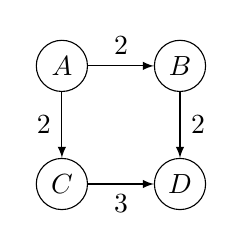
\begin{tikzpicture}[node distance={15mm}, main/.style = {draw, circle, inner sep = 0pt, minimum size = 6.5mm}]
                \node[main] (1) {$A$};
                \node[main] (2) [right of = 1] {$B$};
                \node[main] (3) [below of = 1] {$C$};
                \node[main] (4) [right of = 3] {$D$};
        
                \draw[-latex] (1) -- (2) node[midway,above = 0.5pt] {$2$};
                \draw[-latex] (1) -- (3) node[midway,left = 0.5pt] {$2$};
                \draw[-latex] (2) -- (4) node[midway,right = 0.5pt] {$2$};
                \draw[-latex] (3) -- (4) node[midway,below = 0.5pt] {$3$} (1);
                
            \end{tikzpicture}
            \end{center} 
            \textit{En revanche si $h(but) = 0$ en plus de la monotonie, l'heuristique est admissible donc on trouve bien un plus court chemin.} 
            \item Est polynomial en temps si $h$ est admissible. \textit{Non, potentiellement exponentiel, car un même sommet peut passer plusieurs fois dans la file de priorité avec des priorités différentes.}
            \item \blacktriangleright {Est polynomial en temps si $h$ est monotone.} \textit{Car tout noeud est extrait au plus une fois de la FdP.}
            \item N'est pas intéressant à appliquer sur un graphe non pondéré. \textit{Trouver un plus court chemin en termes de nombre d'arêtes peut être pertinent dans certains contextes.}
        \end{enumerate}
    \item Quelles propriétés sont justes sur les arbres couvrants parmi les suivantes ? 
        \begin{enumerate}
            \item Tout graphe possède un arbre couvrant. \textit{Ce n'est pas le cas pour les graphes non connexes.}
            \item \blacktriangleright {Dans un graphe $G$, tout arbre couvrant de poids minimum (ACM) contient au moins une arête de poids minimal de $G$.} \textit{"sinon, on prend $(s,t)$ une des arêtes de poids minimal ; elles sont reliées dans l'ACM via un chemin qui n'emprunte aucune arête de poids minimal et il suffirait d'enlever une des arêtes de ce chemin et rajouter $(s,t)$ pour avoir un arbre de poids strictement plus petit que celui d'un ACM.}
            \item L'arête de poids maximal n'appartient à aucun ACM. \textit{Considérer un graphe connexe à deux sommet : le seul ACM contient la seule arête qui est de poids maximal.}
            \item \blacktriangleright {Si les poids de toutes les arêtes de $G$ sont deux à deux distincts et que $G$ est connexe alors $G$ admet un unique ACM.} \textit{Montré en exercice.}
            \item Si $G$ admet un unique ACM, les poids de ses arêtes sont deux à deux distincts. \textit{Considérer un graphe connexe à $3$ sommets et $2$ arêtes de même poids.}
        \end{enumerate}
    \item Lesquelles parmi les propriétés suivantes sur les couplages sont vraies ? 
        \begin{enumerate}
            \item Un couplage maximal est maximum. \textit{Contre-exemple vu en cours.}
            \item \blacktriangleright {Un couplage maximum est maximal.}
            \item Un graphe admettant un couplage parfait est nécessairement biparti.
            \item \blacktriangleright {Dans un graphe biparti, on peut calculer un couplage maximal en temps polynomial.} \textit{Oui puisqu'on peut calculer un couplage maximum via l'algorithme de Berge, qui est maximal.}
            \item \blacktriangleright {Un couplage sans chemin augmentant dans un graphe biparti est maximum.} \textit{C'est même vrai dans les graphes qui ne sont pas bipartis : c'est le lemme de Berge.}
        \end{enumerate}
    \item Soient $C_1$, $C_2$ deux couplages d'un graphe $G$. Alors :
        \begin{enumerate}
            \item $C_1 \cup C_2$ est un couplage.
            \item $C_1 \cap C_2$ est un couplage.
            \item \blacktriangleright $C_1 \Delta C_2$ ($C_1 \cup C_2\setminus C_1 \cap C_2$) est un couplage. \textit{On peut trouver des contre-exemples pour les autres}
            \item $C_1 \setminus C_2$ est un couplage.
        \end{enumerate}
    \item L'algorithme des $k$ plus proches voisins ... 
        \begin{enumerate}
            \item Est un algorithme d'apprentissage non supervisé. \textit{Supervisé au contraire.}
            \item Gagne en précision lorsqu'on augmente $k$. \textit{Pas nécessairement, surapprentissage.}
            \item Ne peut pas être acceléré par pré-traitement. \textit{Faux car stocker les données d'entraînement dans un arbre $d$-dimensionnel permet de trouver plus rapidement les $k$ voisins d'un point dont on cherche la classe.}
            \item \blacktriangleright {Aucune des réponses ci-dessus.}
        \end{enumerate}
    \item Un arbre de décision ... 
        \begin{enumerate}
            \item \blacktriangleright {Peut être construit par un algorithme d'apprentissage supervisé.} \textit{ID3 par exemple.}
            \item Classe  toujours correctement tous les éléments de l'ensemble d'apprentissage. \textit{ID3 peut parfois créer des feuilles en considérant la classe majoritaire des exemples correspondants. Si cette classe majoritaire est "oui", les exemples d'entraînement pour lesquels la réponse est "non" seront mal classés.}
            \item Peut être amélioré à l'aide d'arbres k-d. \textit{A priori, non, ça c'est pour les $k$ plus proches voisins.}
            \item Peut être calculé sans calcul d'entropie par l'algorithme ID3. \textit{ID3 utilise justement l'entropie. Mais on pourrait cocher cette réponse car : on peut faire ID3 sans utiliser le critère d'entropie pour séparer les exemples, et on peut construire un arbre de décision sans ID3.}
            \item \blacktriangleright {A une hauteur bornée par la dimension des données.} \textit{On sépare au plus sur chacun des attributs.}
        \end{enumerate}
    \item L'algorithme des $k$ moyennes ... 
        \begin{enumerate}
            \item Repose sur l'entropie de Shannon. \textit{C'est ID3 qui fait ça.}
            \item Converge vers une réponse optimale. \textit{On peut avoir convergence vers un optimum local non global.}
            \item Ne converge pas nécessairement. \textit{Il y a en revanche toujours convergence.}
            \item \blacktriangleright {Ne reconnaît pas les classes non convexes.} \textit{Exemple : deux classes concentriques.}
            \item Nécessite un calcul de médioïde. \textit{Le bon terme est "centroïde".}
        \end{enumerate}
    \item La classification obtenue par un algorithme de regroupement hiérarchique ascendant ... 
        \begin{enumerate}
            \item Est indépendante de la distance choisie.
            \item \blacktriangleright {Permet de choisir le nombre de clusters.} \textit{En coupant à la hauteur voulue.}
            \item Ne reconnaît pas les classes non convexes.
            \item Nécessite un calcul de centroïde.
            \item \blacktriangleright {A une complexité dépendante de la distance considérée.} \textit{Ne serait-ce que parce que la complexité du calcul de cette distance intervient dans la complexité de l'algorithme complet.}
        \end{enumerate}
    \item Un algorithme reposant sur une heuristique ... 
        \begin{enumerate}
            \item Ne peut pas donner une réponse optimale à coup sûr. \textit{Considérer $A^{\star}$ avec une heuristique admissible.}
            \item Ne peut généralement pas garantir le temps d'exécution et l'optimalité du résultat. \textit{$A^{\star}$ avec une heuristique monotone et admissible fournit un contre-exemple. On peut légitimement cocher cette réponse à cause du "généralement".}
            \item Ne peut pas être exécuté avec une heuristique différente.
            \item \blacktriangleright {Peut être ajusté pour une utilisation pratique précise en adaptant l'heuristique considérée.}
            \item Aucune des réponses ci-dessus.
        \end{enumerate}
    \item Les positions gagnantes pour un joueur $J_1$ dans un jeu à deux joueurs ... 
        \begin{enumerate}
            \item \blacktriangleright {Peuvent être calculées en temps polynomial en la taille du jeu.} \textit{Avec l'algorithme des attracteurs, avec programmation dynamique.}
            \item Dépendent des réponses de l'adversaire. \textit{Justement non.}
            \item Sont nécessairement des sommets contrôlés par le joueur $J_1$. \textit{Pas obligatoirement.}
            \item \blacktriangleright {Peuvent mener à une défaite de $J_1$.} \textit{Il suffit que $J_1$ joue autre chose qu'une stratégie gagnante !}
            \item Aucune des réponses ci-dessus.
        \end{enumerate}
\end{enumerate}


\section*{Logique}

\begin{enumerate}[resume]
    \item La formule << ($A\rightarrow B) \leftrightarrow (\lnot A \lor B)$ >> :
    \begin{enumerate}
        \item \blacktriangleright est vraie au sens de la logique propositionnelle
        \item est prouvable dans la logique minimale\textit{on a besoin du tiers exclu pour montrer $A\rightarrow B \vdash \lnot A \lor B$}
        \item \blacktriangleright est prouvable dans la logique classique (en ajoutant tiers exclu ou raa à la logique minimale)
    \end{enumerate}
    \item Quelles formules sont des tautologies ? 
        \begin{enumerate}
            \item $((A \Rightarrow B) \Rightarrow C) \Leftrightarrow (A \Rightarrow (B \Rightarrow C))$. \textit{Rendue fausse par $v(A) = v(B) = v(C) = 0$.}
            \item $(A \lor B) \wedge (\neg A \lor \neg B)$. \textit{Est rendue fausse par $v(A) = v(B) = 0$.}
            \item \blacktriangleright ${\neg(A \wedge (A \lor B)) \Leftrightarrow \neg A}$. \textit{Il suffit de faire une disjonction de cas selon $v(A)$.}
            \item $((A \lor B) \wedge (C \lor D)) \Leftrightarrow (A \wedge B)\lor(B \wedge D)$. \textit{Aucune chance.}
            \item \blacktriangleright ${(A \Rightarrow B) \Leftrightarrow (\neg A \lor B)}$. \textit{Vrai vu l'équivalence classique $A \Rightarrow B \equiv \neg A \lor B$.}
        \end{enumerate}
    \item La taille d'une formule est majorée par sa hauteur. 
        \begin{enumerate}
            \item Vrai.
            \item \blacktriangleright {Faux.} \textit{C'est la hauteur d'un arbre qui est majorée par sa taille.}
        \end{enumerate}
    \item Une variable libre ... 
        \begin{enumerate}
            \item \blacktriangleright {Peut être liée à un autre endroit dans la formule.} \textit{Techniquement c'est plutôt une occurrence de cette variable qui peut être liée à un autre endroit.}
            \item A une portée. \textit{Ce sont les quantificateurs qui ont une portée.}
            \item N'influe pas la sémantique d'une formule.
            \item Est toujours associée à une variable liée.
        \end{enumerate}
    \item Soit $\varphi$ et $\psi$ deux formules telles que $\psi \models \varphi$. Cela signifie ... 
        \begin{enumerate}
            \item \blacktriangleright {Que $\varphi$ est conséquence de $\psi$.}
            \item Que $\psi$ est conséquence de $\varphi$.
            \item Que les valuations satisfaisant $\varphi$ satisfont aussi $\psi$. \textit{C'est l'inverse.}
            \item \blacktriangleright {Si $\varphi$ est une antilogie, alors $\psi$ aussi.} \textit{Si une valuation satisfaisait $\psi$, elle satisferait $\varphi$ ce qui n'est pas.}
            \item Cela n'a pas de sens, la notation $\models$ n'existe que sous la forme $v \models \varphi$ avec $v$ une valuation.
        \end{enumerate}
    \item Une équivalence entre formules du calcul propositionnel ... 
        \begin{enumerate}
            \item Signifie qu'elles ont le même arbre de dérivation. 
            \item \blacktriangleright {Peut se prouver à l'aide de tables de vérité.}
            \item \blacktriangleright {Peut se prouver à l'aide de substitutions dans des formules qu'on sait déjà être équivalentes.}
            \item Ne peut pas être démontrée sans la déduction naturelle. \textit{Si, avec un raisonnement sémantique.}
            \item Peut se prouver par une étude de la matrice de confusion.
        \end{enumerate}
    \item Pour toute formule du calcul du calcul propositionnel il existe une formule équivalente ...
        \begin{enumerate}
            \item \blacktriangleright {Sous forme normale conjonctive.}
            \item \blacktriangleright {Sous forme normale disjonctive.}
            \item Sous forme normale de Quine. \textit{L'algorithme de Quine calcule la satisfiabilité d'une formule.}
            \item Sous forme normale littérale.
            \item Sous forme normale de Chomsky. \textit{ça c'est pour les grammaires algébriques.}
            \item Aucune des réponses précédentes.
        \end{enumerate}
    \item On sait résoudre le problème SAT en temps polynomial sur des instances ... 
        \begin{enumerate}
            \item \blacktriangleright {Sous $2$-CNF.} \textit{Via Kosaraju ou DPLL.}
            \item Sous $3$-CNF. \textit{A priori non par NP-complétude de \texttt{3-SAT}.}
            \item \blacktriangleright {Sous $2$-DNF.} \textit{La satisfiabilité d'un formule sous DNF se décide toujours polynomialement : il suffit de parcourir chaque clause et d'observer si l'une au moins ne contient pas un littéral et sa négation.}
            \item \blacktriangleright {Sous $3$-DNF.}
            \item Ne faisant intervenir que les connecteurs $\wedge$ et $\neg$.
        \end{enumerate}
    \item Quels séquents sont prouvables en logique classique ? \textit{Il suffit de regarder si le séquent est valide : si oui, il est prouvable et sinon non. Il n'y a donc pas besoin de chercher des arbres de preuve pour cette question.}\begin{multicols}{2}
        \begin{enumerate}
            \item \blacktriangleright ${\neg \neg A \vdash A}$.
            \item \blacktriangleright ${\neg \neg \neg A \vdash \neg A}$.
            \item \blacktriangleright ${A \wedge B \vdash A \lor B}$.
            \item $A \lor B \vdash A \wedge B$.
            \item \blacktriangleright ${A, A \rightarrow B \vdash B}$.
        \end{enumerate}
        \end{multicols}
    \item Pour la déduction naturelle en logique propositionnelle, $\Gamma \vdash F$ si et seulement si $\Gamma \models F$. 
        \begin{enumerate}
            \item \blacktriangleright {Vrai.} \textit{La déduction naturelle est correcte et complète (HP).}
            \item Faux.
        \end{enumerate}
\end{enumerate}


\section*{Théorie des langages}

\begin{enumerate}[resume]
    \item Sur l'aphabet $\Sigma = \{a, b\}$ :
        \begin{enumerate}
            \item $\emptyset$ est une lettre.
            \item $\emptyset$ est un mot.
            \item \blacktriangleright $\emptyset$ est un langage.
            \item $\epsilon$ est une lettre.
            \item \blacktriangleright $\epsilon$ est un mot.
            \item \blacktriangleright $\epsilon$ est un langage.\textit{Le langage contenant seulement le mot $\epsilon$}
        \end{enumerate}
    \item Si $u$ et $v$ sont deux mots, quelles propriétés parmi les suivantes sont vraies ? 
        \begin{enumerate}
            \item $|u| >0$. \textit{On pourrait avoir $u = \varepsilon$.}
            \item $u$ est préfixe de $v$ ou $v$ est préfixe de $u$. \textit{Contre-exemple avec $u = a$ et $v = b$.}
            \item Si $u$ est préfixe de $v$ alors $v$ est suffixe de $u$. \textit{Contre-exemple : $u = a$ est préfixe de $v = ab$.}
            \item \blacktriangleright {Si $u = vw$ alors $v$ est un sous-mot de $u$.} \textit{C'en est même un préfixe.}
            \item \blacktriangleright {Si $u = vw$ alors $v$ est un facteur de $u$.} \textit{C'en est même un préfixe.}
        \end{enumerate}
    \item Si $L$, $L'$ et $L''$ sont des langages alors ... 
        \begin{enumerate}
            \item Si $L$ et $L'$ sont finis, $|LL'| = |L|\times|L'|$. \textit{Contre-exemple : $L = \{\varepsilon,a \}$ et $L' = \{b,ab\}$. On a $LL' = \{b, ab, aab\}$ qui n'est pas de taille $4$. On peut obtenir le même mot avec plusieurs concaténations différentes.}
            \item $L^{\star}$ est infini. \textit{Pas si $L = \{ \varepsilon \}$.}
            \item $L \subset LL$. \textit{Contre-exemple : $L = \{a\}$ ; on a alors $LL = \{aa\}$. Fonctionne ssi $L$ contienne $\varepsilon$.}
            \item $L(L' \cap L'') = LL' \cap LL''$. \textit{Contre-exemple : $L = \{a, ab\}$, $L' = \{\varepsilon\}$, $L'' = \{b\}$ car $\emptyset \neq \{ab \}$. }
            \item \blacktriangleright {Aucune des réponses précédentes.}
        \end{enumerate}
    \item Si $L$ et $L'$ sont deux langages tels que $L \subset L'$ , quelles affirmations sont vraies ? 
        \begin{enumerate}
            \item Si $L'$ est reconnaissable alors $L$ aussi. \textit{Contre-exemple : $L = \{a^nb^n \, | \, n \in \mathbb{N} \}$ et $L' = (a|b)^{\star}$.}
            \item Si $L'$ n'est pas rationnel, $L$ non plus. \textit{Contre-exemple : $L' = \{a^nb^n \, | \, n \in \mathbb{N} \}$ et $L = \{\varepsilon \}$. }
            \item \blacktriangleright {Si $L'$ est fini, $L$ est rationnel.} \textit{Car alors $L$ est fini donc rationnel.}
            \item \blacktriangleright {Si $L$ est reconnaissable, il l'est par un automate déterministe et complet.} \textit{Si $L$ est reconnaissable par un automate, on peut déterminiser et compléter ce dernier.}
            \item Si $L$ est reconnaissable, il l'est par un automate émondé et complet. \textit{On ne peut pas garantir le caractère à la fois émondé et complet, par exemple avec $L = \{a\}$ sur l'alphabet $\{a,b\}$.}
        \end{enumerate}
    \item Le langage $L = \{a^nb^m \, | \, n \equiv m \text{ mod }  2 \}$ est dénoté par l'expression régulière ... \textit{Ce langage est bien rationnel et est dénoté entre autres par $(a^2)^{\star}(b^2)^{\star} | a(a^2)^{\star}b(b^2)^{\star}$ : soit les exposants sont pairs tous les deux, soit impairs.}
        \begin{enumerate}
            \item $(aa|bb)^{\star}$. \textit{$aabbaa$ est dans ce langage mais pas dans $L$.}
            \item $(aa|ab|ba|bb)^{\star}$. \textit{$abba$ est dans ce langage mais pas dans $L$.}
            \item $((a(a|b)^{\star}b)^{\star}+(b(a|b)^{\star}a)^{\star})^{\star}$. \textit{$abab$ est dans ce langage mais pas dans $L$.}
            \item $a^nb^m$. \textit{N'a pas de sens : qui sont $m$ et $n$ ?}
            \item \blacktriangleright {Aucune des réponses précédentes.}
        \end{enumerate}
    \item Les langages rationnels sont stables par ... 
        \begin{enumerate}
            \item \blacktriangleright {Préfixe.} \textit{\'Emonder un automate qui reconnaît $L$ et rendre tous ses états finaux.}
            \item \blacktriangleright {Miroir.} \textit{Changer le sens des transitions d'un automate qui reconnaît $L$, les initiaux deviennent finaux et les finaux initiaux.}
            \item \blacktriangleright {Complémentaire.} \textit{On calcule un automate déterministe et complet (les deux sont importants) pour $L$ puis les finaux deviennent non finaux et les non finaux deviennent finaux.}
            \item \blacktriangleright {Intersection.} \textit{Via la construction de l'automate produit.}
        \end{enumerate}
    \item Un automate fini déterministe et complet ... 
        \begin{enumerate}
            \item Est nécessairement émondé. \textit{Contre-exemple : Un automate qui reconnaît $\{a\}$ sur $\{a,b\}$ avec un puits.}
            \item Est unique pour chaque langage à renommage près des états. \textit{C'est vrai dans le cadre d'un automate minimal. Pour un automate quelconque, on peut toujours rajouter des états inutiles.}
            \item \blacktriangleright {Permet de tester l'appartenance d'un mot à un langage en temps linéaire.} \textit{Il suffit de lire toutes les lettres du mot et il n'y a qu'un seul chemin à explorer par déterminisme.}
            \item \blacktriangleright {Donne aisément un automate reconnaissant le complémentaire du langage.} \textit{En inversant finaux et non finaux. Attention cette transformation ne marche pas si l'automate n'est pas déterministe et complet.}
            \item Est de taille exponentielle en la taille d'un automate non déterministe reconnaissant le même langage. \textit{Pas nécessairement, même si au pire cas ça peut arriver.}
        \end{enumerate}
    \item Si $e$ est une expression rationnelle, le problème consistant à savoir si un mot $u$ appartient à $L(e)$ ... 
        \begin{enumerate}
            \item \blacktriangleright {Nécessite au moins une complexité linéaire en $|u|$.} \textit{Il faut a priori lire le mot. On peut ne pas cocher cette réponse à cause du "nécessite" : si $e = \emptyset$ par exemple, il n'y a pas besoin de lire le mot.}
            \item \blacktriangleright {Peut être résolu en temps polynomial en $|u|+|e|$.} \textit{Construire un automate $A$ non déterministe qui reconnaît $L(e)$ se fait polynomialement en $|e|$ via l'algorithme de Berry-Sethi. Cet automate a au plus de l'ordre de $|e|$ états et il y a au plus $|e|$ transitions par état. La lecture de $u$ dans $A$ est aussi polynomiale en $|e|$ et $|u|$ : il suffit de garder en mémoire l'ensemble d'états (au plus $n$) dans lequel on peut être après lecture de chacune des au plus $|u|$ lettres de $u$, et lire une lettre consiste à examiner au plus $|e|$ transitions pour un coût majoré par $O(|u||e|^2)$.}
            \item Est un problème indécidable. \textit{Non : cf (B).}
            \item N'a pas d'application pratique. \textit{Ne serait-ce que la reconnaissance de motif.}
            \item Aucune des réponses précédentes.
        \end{enumerate}
    \item Tout automate est équivalent à...
        \begin{enumerate}
            \item un automate déterministe, construit en complexité polynomiale.\textit{complexité exponentielle car $2^n$ états dans l'automate des parties}
            \item \blacktriangleright un automate complet.
            \item \blacktriangleright un automate déterministe complet.\textit{algorithme de déterminisation}
            \item un automate déterministe complet émondé.\textit{rendre l'automate demande d'avoir un état << poubelle >> qui n'est pas co-accessible}
            \item \blacktriangleright un automate sans $\epsilon$-transition.
        \end{enumerate}
    \item Un automate produit de deux automates $A_1$ et $A_2$ d'états $Q_1$ et $Q_2$...
        \begin{enumerate}
            \item \blacktriangleright possède $Q_1\times Q_2$ comme ensemble d'états.
            \item peut permettre de reconnaître $L(A_1)L(A_2)$.
            \item \blacktriangleright peut permettre de reconnaître $L(A_1)\cup L(A_2)$.
            \item \blacktriangleright peut permettre de reconnaître $L(A_1)\cap L(A_2)$.
            \item \blacktriangleright peut permettre de reconnaître $L(A_1)\setminus L(A_2)$.
            \item \blacktriangleright peut permettre de reconnaître $L(A_1)\Delta L(A_2)$.
        \end{enumerate}
    \item On peut montrer que tout langage rationnel est reconnaissable par un automate fini ... 
        \begin{enumerate}
            \item En construisant l'automate des parties. \textit{Permet de déterminiser un automate.}
            \item \blacktriangleright {En utilisant les automates de Thompson.}
            \item En utilisant la méthode d'élimination des états. \textit{Permet de faire la réciproque, à savoir montrer qu'un langage reconnu est dénoté par un expression rationnelle.}
            \item Avec l'algorithme de McNaughton Yamada. \textit{Idem (C).}
            \item \blacktriangleright {En utilisant l'algorithme de Berry-Sethi.}
        \end{enumerate}
    \item Parmi les langages suivants, lesquels sont réguliers ? 
        \begin{enumerate}
            \item $\{a^nb^n \, | \, n \geq 0\}$. \textit{Preuve par l'absurde avec le lemme de l'étoile.}
            \item Les mots bien parenthésés. \textit{Preuve par l'absurde avec le lemme de l'étoile.}
            \item \blacktriangleright ${\{a^nb^m \, | \, n \equiv m \text{ mod } 2 \}}$.  \textit{Cf question 62. Ou faire un automate à $4$ états.}
            \item \blacktriangleright {Les mots sur $\{0,1\}$ correspondant aux écritures binaires d'entiers divisibles par $3$.} \textit{Cf exemple introductif du cours où les états indiquent les restes possibles modulos $3$.}
            \item $\{a^p \, | \, p \text{ est premier} \}$. \textit{Preuve par l'absurde avec le lemme de l'étoile.}
        \end{enumerate}
    \item Un langage $L$ est local ssi...
        \begin{enumerate}
            \item \blacktriangleright {$L$ est reconnu par un automate local.}
            \item $L$ est inclus dans un langage régulier.
            \item \blacktriangleright $L\backslash \{\epsilon\} = P(L) \Sigma^* \cap \Sigma^* S(L) \backslash \Sigma^* N(L) \Sigma^*$ où $N(L) = \Sigma^2 \backslash F(L)$.
            \item \blacktriangleright $u \in L ~\Longleftrightarrow ~u_1 \in P(L) \wedge u_n \in S(L) \wedge \forall k, u_k u_{k+1} \in F(L)$
        \end{enumerate}
    \item Parmi les conditions suivantes, lesquelles sont suffisantes pour que $L$ soit rationnel ? 
        \begin{enumerate}
            \item $L$ est dénombrable. \textit{Contre-exemple : $L = \{a^nb^n \, | \, n \in \mathbb{N}\}$.}
            \item \blacktriangleright {$L$ est reconnu par un automate non déterministe.}
            \item \blacktriangleright {$L$ est le complémentaire d'un langage rationnel.} \textit{Par stabilité des rationnels par complémentaire.}
            \item $L^{\star}$ est rationnel. \textit{Contre-exemple : $L = \{a^p \, | \, p \text{ est premier} \}$ puisque $L^{\star} = a^{\star}$ est rationnel.}
            \item $L \subset \{a\}^{\star}$. \textit{Contre-exemple : $L = \{a^p \, | \, p \text{ est premier} \}$.}
            \item \blacktriangleright {$L$ est local.}
        \end{enumerate}
    \item Si un langage vérifie le lemme de l'étoile, alors il est rationnel. \begin{multicols}{2}
        \begin{enumerate}
            \item Vrai.
            \item \blacktriangleright {Faux.} \textit{Le lemme de l'étoile est une implication.}
        \end{enumerate}
        \end{multicols}
    \item Les langages algébriques ... 
        \begin{enumerate}
            \item Sont inclus dans les langages rationnels. \textit{L'inclusion réciproque est vraie.}
            \item \blacktriangleright {Sont stables par étoile de Kleene.}
            \item Sont stables par complémentaire. \textit{Si c'était le cas, la stabilité par union ferait qu'on a la stabilité par intersection ce qui n'est pas d'après le contre-exemple suivant.}
            \item Sont stables par intersection. \textit{$\{a^nb^nc^m \, | \, n,m \in \mathbb{N}\}$ et $\{a^mb^nc^n \, | \, n,m \in \mathbb{N} \}$ (le premier est engendré par $S \rightarrow ZC, C \rightarrow cC | \varepsilon, Z \rightarrow AZB \, \varepsilon, A \rightarrow a, B \rightarrow b $) sont algébriques mais pas leur intersection $\{a^nb^nc^n \, | \, n \in \mathbb{N} \}$. }
            \item \blacktriangleright {Sont stables par concaténation.}
        \end{enumerate}
    \item Quelles sont les grammaires ambiguës ? 
        \begin{enumerate}
            \item \blacktriangleright ${S \rightarrow SS \, | \, a}$. \textit{Via le mot $aaa$.} 
            \item $S \rightarrow ST \, | \, TS$, $T \rightarrow SS$. \textit{Engendre $\emptyset$ donc il est vrai que tout mot engendré par cette grammaire admet un seul arbre de dérivation, d'après les merveilleuses propriétés de l'ensemble vide.}
            \item \blacktriangleright ${S \rightarrow aSbS \, | \, bSaS \, | \, \varepsilon}$. \textit{Via le mot $abab$.}
            \item \blacktriangleright ${S \rightarrow aSb \, | \, ab \, | \, \varepsilon}$. \textit{Via le mot $ab$.}
            \item $S \rightarrow a S \, | \, bS \, | \, \varepsilon$. \textit{Car il n'y a jamais le choix sur comment dériver.}
        \end{enumerate}
    \item Les dérivations droites sont en bijection avec les arbres de dérivation. \textit{Au sens où si on se donne $G$ et $u \in L(G)$, il y a bijection entre les arbres de dérivation pour $u$ et les dérivations droites pour $u$. En effet, si on a un arbre, il donne une dérivation droite ; celle consistant à appliquer les règles telles que rencontrées dans un parcours en profondeur de l'arbre effectué de droite à gauche. Une dérivation droite donne immédiatement un arbre.}\begin{multicols}{2}
        \begin{enumerate}
            \item \blacktriangleright {Vrai.}
            \item Faux.
        \end{enumerate}
        \end{multicols}
    \item Un analyseur lexical ... 
        \begin{enumerate}
            \item \blacktriangleright {Intervient avant l'analyseur syntaxique.}
            \item \blacktriangleright {Identifie les lexèmes.}
            \item Permet de déterminer la structure d'un programme. \textit{C'est le rôle de l'analyse syntaxique.}
            \item \blacktriangleright {Peut utiliser un automate fini.} \textit{Pour reconnaître les mots qui sont des lexèmes.}
        \end{enumerate}
    \item Un analyseur syntaxique ... 
        \begin{enumerate}
            \item Ne peut gérer que des grammaires non ambiguës. \textit{Non, c'est juste plus délicat.}
            \item \blacktriangleright {Considère les lexèmes comme des terminaux.}
            \item N'est pas utilisé en pratique. \textit{Si, dans les compilateurs par exemple.}
            \item Choisit la grammaire à considérer en fonction des données en entrée. \textit{N'a pas de sens.}
            \item Aucune des réponses précédentes.
        \end{enumerate}
\end{enumerate}


\section*{Complexité et calculabilité}

\begin{enumerate}[resume]
    \item Parmi les problèmes ci-dessous, lesquels sont des problèmes de décision ? 
        \begin{enumerate}
            \item La résolution d'une grille de Sudoku.
            \item \blacktriangleright {La primalité d'un entier.}
            \item Le plus court chemin entre deux points.
            \item \blacktriangleright {Le problème de l'arrêt.}
            \item \blacktriangleright {L'égalité entre deux langages.}
        \end{enumerate}
    \item Parmi les problèmes ci-dessous, lesquels sont des problèmes d'optimisation ? 
        \begin{enumerate}
            \item La résolution d'une grille de Sudoku. \textit{On pourrait argumenter que ce problème est celui consistant à minimiser le nombre d'incohérences (deux mêmes chiffres sur la même ligne, colonne, carré) dans une grille complète qui respete celle en entrée. Mais c'est un peu abusif car a priori, résoudre un Sudoku veut plutôt dire : trouver une solution correcte ou affirmer qu'il n'y en a pas.}
            \item La primalité d'un entier.
            \item \blacktriangleright {Le plus court chemin entre deux points.}
            \item Le problème de l'arrêt.
            \item L'égalité entre deux langages.
        \end{enumerate}
    \item Si $n$ est la taille de l'entrée, pour quelles complexités peut-on dire que l'algorithme considéré est polynomial ?
        \begin{enumerate}
            \item \blacktriangleright ${O(\log n!)}$. \textit{Car ceci est un $O(n \log n) = O(n^2)$}
            \item $2^{o(n)}$. \textit{On a $(\log n)^2 = o(n)$ et si on avait $2^{(\log n)^2 } \leq n^k$ pour un certain $k$, on aurait $(\log n)^2 / \log n \leq k$.}
            \item $O((\log n)^n)$. \textit{S'il existe $k$ tel que $(\log n)^n \leq n^k$, on aurait $n \log \log n \leq k \log n$ : contradiction à l'infini. }
            \item \blacktriangleright ${O(\sqrt{n})}$. \textit{C'est par exemple un $O(n)$.}
            \item $O(2^n)$. \textit{Est évidemment exponentiel en $n$.}
        \end{enumerate}
    \item L'algorithme cherchant à déterminer si un entier $n$ est premier en calculant son modulo par tous les entiers entre $2$ et $\lceil \sqrt{n} \rceil$ est de complexité ...
        \begin{enumerate}
            \item Quasi-linéaire.
            \item Polynomiale. \textit{Non car la taille de l'entier $n$ est $\log n$ donc $O(\sqrt{n}) = O(\sqrt{e}^{\log n})$.}
            \item Sous-linéaire.
            \item \blacktriangleright {Exponentielle.}
            \item Linéaire. \textit{Cette réponse, ainsi que (A) et (C) sont fausses vu (B).}
        \end{enumerate}
    \item La complexité d'un problème de décision correspond à ... 
        \begin{enumerate}
            \item \blacktriangleright {La complexité pire cas du meilleur algorithme qui le résout.} \textit{On pourrait ne pas cocher cet item car la notion de "meilleur algorithme" est trop floue. Un algorithme peut être dans plusieurs classes de complexité différentes selon le type d'algorithme pour le résoudre considéré.}
            \item La complexité pire cas du pire algorithme qui le résout.
            \item La complexité meilleur cas du meilleur algorithme qui le résout.
            \item \blacktriangleright {Dépend du format d'entrée des instances.}
            \item N'est pas définie.
        \end{enumerate}
    \item On suppose que $A$ est NP-complet. Soit $B\in$ NP. Pour montrer que $B$ est NP-complet, il suffit de montrer... \begin{multicols}{2}
        \begin{enumerate}
            \item \blacktriangleright {$A$ se réduit polynomialement à $B$.}
            \item $B$ se réduit polynomialement à $A$.
            \item \blacktriangleright {$A \leq_p B$.}
            \item $B \leq_p A$.
            \item \blacktriangleright {À chaque instance $I_A$ de $A$, on peut associer une instance $I_B$ de $B$ en temps polynomial telle que $I_A$ est une instance positive de $A$ ssi $I_B$ est une instance positive de $B$.}
            \item À chaque instance $I_B$ de $B$, on peut associer une instance $I_A$ de $A$ en temps polynomial telle que $I_A$ est une instance positive de $A$ ssi $I_B$ est une instance positive de $B$.
        \end{enumerate}
        \end{multicols}
    \item Si le problème $A$ se réduit polynomialement au problème $B$ alors ... 
        \begin{enumerate}
            \item Si $A$ se résout en temps polynomial, $B$ aussi. \textit{Tout problème dans P est NP donc se réduit à \texttt{SAT}.}
            \item \blacktriangleright {Si $B$ se résout en temps polynomial, $A$ aussi.}
            \item $A$ est considéré comme plus difficile que $B$. \textit{Non, c'est l'inverse.}
            \item \blacktriangleright {Une instance de $A$ peut être transformée en une instance de $B$.} \textit{Dans le cadre de réductions many-one.}
            \item Si $A$ est décidable alors $B$ aussi.
        \end{enumerate}
    \item Si un problème est dans NP alors ...
        \begin{enumerate}
            \item On ne sait pas le résoudre en temps polynomial. \textit{Tout problème P est dans NP.}
            \item \blacktriangleright {Il peut être résolu en temps exponentiel.}
            \item \blacktriangleright {Il peut être résolu en espace polynomial.} \textit{Si $A$ est dans NP, il existe un ensemble de certificats $C$ et un problème $B \in$ P tel que $x$ est une instance positive de $A$ ssi il existe $c \in C$ de taille polynomiale en $|x|$ tel que $(x,c)$ est positive pour $B$. Un algorithme pour savoir si $x$ est positive pour $A$ consiste donc à parcourir tous les certificats et utiliser un algo polynomial pour $B$. Pour chaque certifiat on utilise un temps donc un espace polynomial et on réutilise le même espace pour stocker le certificat suivant.}
            \item Il s'agit d'un problème fonctionnel.
            \item Pour toute instance du problème, on peut créer un certificat en temps polynomial. \textit{Si on savait faire ça, on aurait P = NP. Pour un problème NP on sait juste qu'il existe un certificat pour toute instance positive et que la vérification qu'un certificat en est bien un se fait en temps polynomial}
        \end{enumerate}
    \item Lesquels de problèmes suivants sont NP-complets ? 
        \begin{enumerate}
            \item \blacktriangleright {\texttt{3SAT}.}
            \item Le problème de l'arrêt. \textit{Il n'est même pas décidable.}
            \item \blacktriangleright {L'existence d'un chemin hamiltonien.}
            \item L'appartenance d'un mot à un langage régulier. \textit{Non, cf partie langages.}
            \item \blacktriangleright {Le problème CLIQUE.}
        \end{enumerate}
    \item Les problèmes indécidables ... 
        \begin{enumerate}
            \item Ne sont pas les mêmes suivant le langage de programmation choisi. \textit{Techniquement c'est vrai, dès lors qu'on considère un langage Turing-complet et un qui ne l'est pas.}
            \item Ne peuvent pas être réduits à un autre problème.
            \item Dépendent de la façon dont sont représentées les instances du problème. \textit{En revanche la complexité d'un algorithme qui résout un problème décidable dépend de la façon dont sont représentées les instances.}
            \item Ne concernent que des problèmes se rapportant au fonctionnement d'algorithmes. \textit{Non, par exemple, déterminer si une grammaire algébrique est ambiguë est indécidable.}
            \item \blacktriangleright {Aucune des réponses précédentes.}
        \end{enumerate}
    \item Parmi les suivants, quels sont les problèmes indécidables ? 
        \begin{enumerate}
            \item \blacktriangleright {Le problème de l'arrêt sur les entrées de taille inférieure à $5$.} %\textit{On ne peut pas entrelacer les exécutions sur toutes les entrées de taille plus petite que 5 car il peut y en avoir une infinité et on ne peut pas non plus lancer séquentiellement ces exécutions}.
            \item Le problème de la terminaison en moins de $n$ étapes sur toute instance de taille inférieure à $n$. \textit{Il suffit d'exécuter $n$ étapes de calcul (en $O(n)$) et de regarder si c'est fini.}
            \item \blacktriangleright {Le problème de la terminaison en strictement plus de $n$ étapes sur toute instance de taille inférieure à $n$.} %TODO
            \item Le problème de l'équivalence de deux expressions régulières. \textit{Il suffit de faire des automates pour les deux, d'en construire la différence symétrique et de vérifier si le langage reconnu est vide.}
            \item Le problème de l'équivalence entre deux formules du calcul propositionnel. \textit{Il suffit de faire leurs tables de vérité.}
        \end{enumerate}
\end{enumerate}
\end{multicols}
\end{document}
